\section{Descrizione architettura}

% Nell'indice proposto da Tullio c'è:
% a. Metodo e formalismo di specifica
% b. Presentazione dell'architettura generale del sistema e identificazione dei componenti architetturali di alto livello

\subsection{Formalismo di specifica}

I diagrammi dei package e delle classi presentati di seguito utilizzano la specifica \glossario{UML} 2.0.

\subsection{Architettura generale}

\begin{figure}[H]
\centering
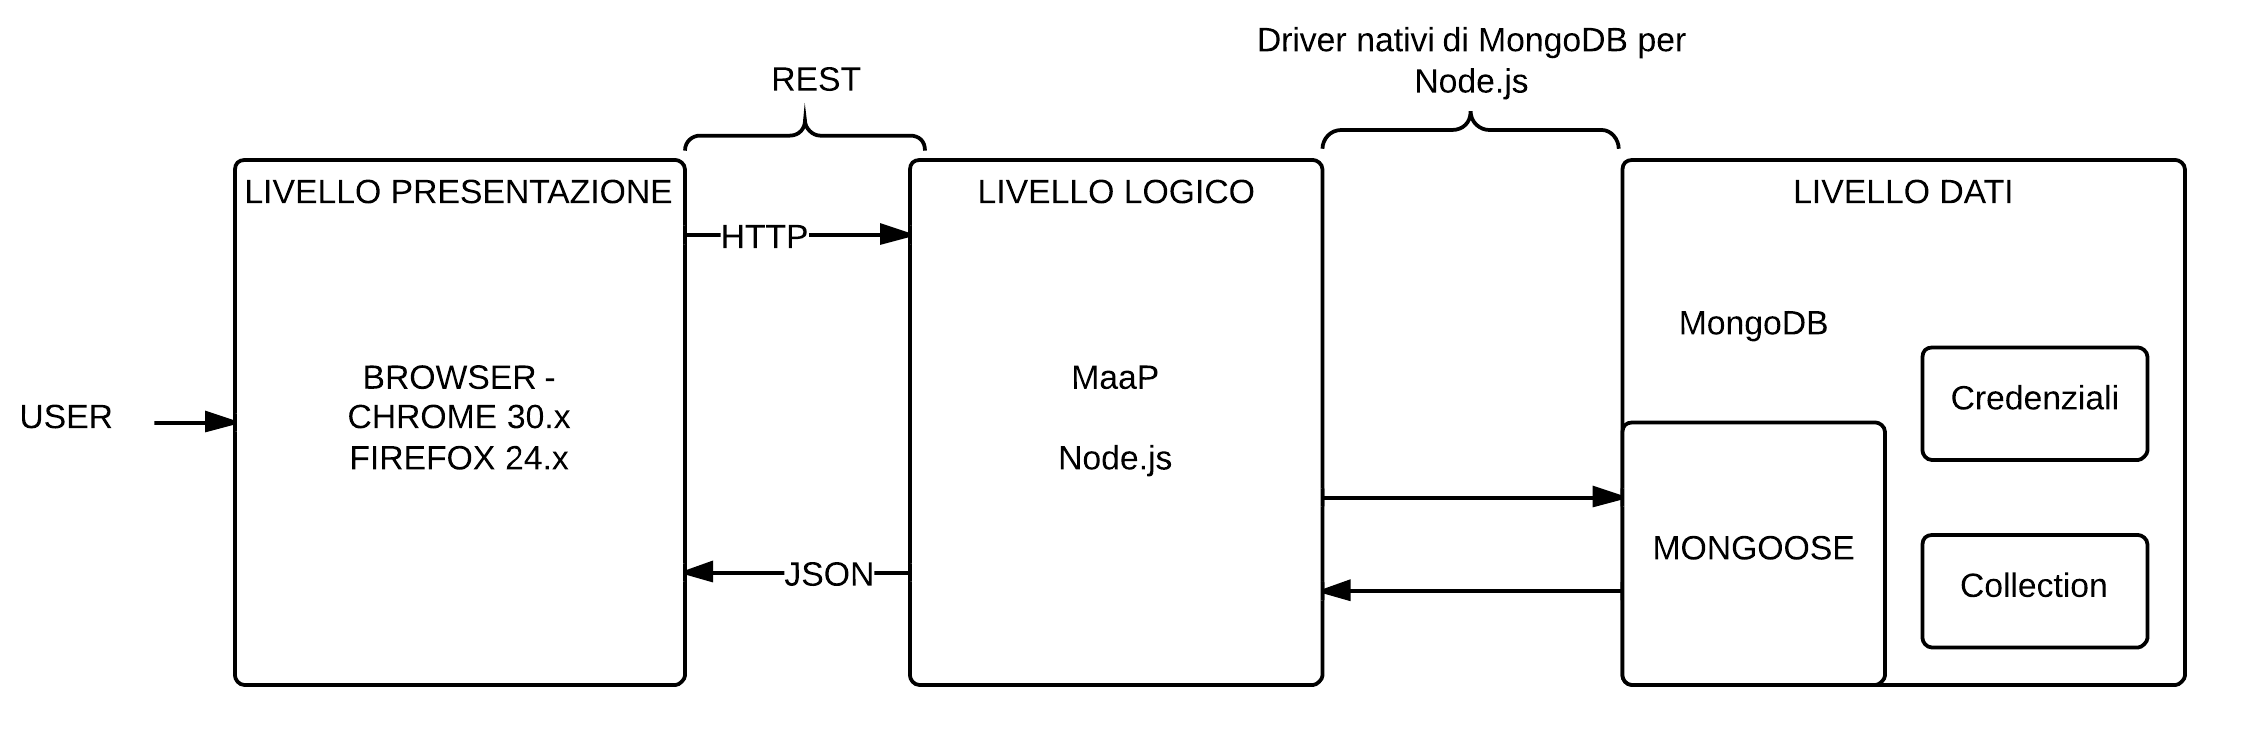
\includegraphics[scale=0.2]{3-TIER.png}
\caption{Schema del modello utilizzato \label{fig:architetturadisistema}}
\end{figure}

\subsection{Three-Tier Architecture}

\emph{Nota: Di seguito i termini modulo, strato e livello sono utilizzati come traduzione del termine inglese tier.}
 
Si tratta di un'architettura di tipo \glossario{client-server}, in cui i processi logici, la persistenza dei dati e l'interfaccia utente sono sviluppati e mantenuti in moduli tra loro indipendenti e distribuiti. Il vantaggio che ne consegue è che un modulo può essere aggiornato o sostituito senza dover alterare gli altri.

Come da figura \ref{fig:architetturadisistema} i tre livelli sono:
\begin{itemize}
\item \textbf{Livello presentazione} Si tratta dello strato che comunica con l'utente, il quale è estraneo all'esistenza degli altri moduli. Il compito di questo strato è fornire un'interfaccia utente, la quale comunicherà con il modulo logico per aggiornarsi e trasmettere le scelte dell'utente. Solitamente questo livello si trova sul \glossario{client};
\item \textbf{Livello logico} Questo livello racchiude le funzionalità, i processi e gli algoritmi dell'applicazione. Solitamente questo livello si trova su un \glossario{server} e si rapporta con il livello interfaccia e il livello dati; 
\item \textbf{Livello dati} In questo livello solitamente si trovano le \glossario{basi di dati}, che garantiscono la persistenza dei dati. È accessibile solo attraverso il livello logico, che ne garantisce la consistenza. In questo livello si trovano anche i componenti utili all'accesso della \glossario{base di dati}, nel nostro caso \glossario{Mongoose}.
E' importante far notare che uno strato dati può comunicare con più strati logici, che potranno utilizzare i dati in maniera diversa.
\end{itemize}

\glossario{Three-Tier} è l'architettura software scelta per \ProjectName.

\subsubsection{\glossario{REST}}

REST, ovvero Representational State Transfer è un tipo di \glossario{RPC}. Si basa su un protocollo di comunicazione \glossario{stateless} di tipo client-server, e solitamente tale protocollo è \glossario{HTTP}, che è stato scelto anche per \ProjectName.

I motivi che hanno spinto alla scelta di REST sono:
\begin{itemize}
\item Semplicità di utilizzo;
\item Indipendenza dal sistema operativo utilizzato dal \glossario{client};
\item Indipendenza dai linguaggi di programmazione utilizzati;
%\item In coppia con HTTPS permette una certa sicurezza delle comunicazioni.
\end{itemize}

\glossario{REST} utilizza il concetto di risorsa, ovvero un aggregato di dati con un nome (\glossario{URI}) e una rappresentazione, su cui è possibile invocare le operazioni \glossario{CRUD} tramite il protocollo sopracitato.

Nell'\glossario{URI} inviato sono presenti il nome della risorsa e la sua rappresentazione, identificata dall'estensione del file scelto, e per \ProjectName è stato scelto il formato \glossario{JSON}, in quanto il suo \glossario{parsing} in \glossario{JavaScript} è più semplice rispetto, ad esempio, quello di \glossario{XML} o \glossario{CSV}.

Un'altra caratteristica di \glossario{REST} è che essendo \glossario{stateless} ogni richiesta dovrà contenere tutte le informazioni necessarie e non dipende dallo stato del sistema.